\section{Introduction}
\label{sec:introduction}


% 1.videoQA overview-----------------------------------------
% 第一段介绍背景:
% 一句话介绍VideoQA的重要性;
% 一句话介绍VideoQA的task;
% 然后引出现有VideoQA models都是black-box的困扰;
% 2-3句话介绍black-box的坏处是啥。

\wx{Video Question Answering (VideoQA) \cite{fan2019heterogeneous} is a keystone in interactive AI, such as vision-language navigation and communication systems.
It aims to answer the natural language question based on the video content.}


In pursuance of interactive AI, Video Question Answering (VideoQA) \cite{fan2019heterogeneous} serves as a keystone in abridging human cognition and machine intelligence, whose goal is to answer the natural language question based on the video content.   
%
Nourished by its multi-modal nature, VideoQA \textit{per se} has relished an overwhelming expansion in model design, which either fosters the vision-language alignment \cite{jiang2020reasoning,park2021bridge} or revisit the visual input structure \cite{le2021hierarchical,dang2021hierarchical}.
%
Albeit their sterling performance, existing solutions are usually expressed as black boxes, where the intrinsic rationale --- how to identify the question-responsive visual elements, is still clouded from our intuition. 
%
As a result, such opaqueness certainly raises reliability concern when the model is deployed in the real-word application, such as \ie intelligent surveillant assistant or more generally, an out-of-distribution test setting.

% More frustratingly, the system gives
% no hint about which part of such systems is the
% culprit for a wrong answer

\begin{figure}[t]
\centering
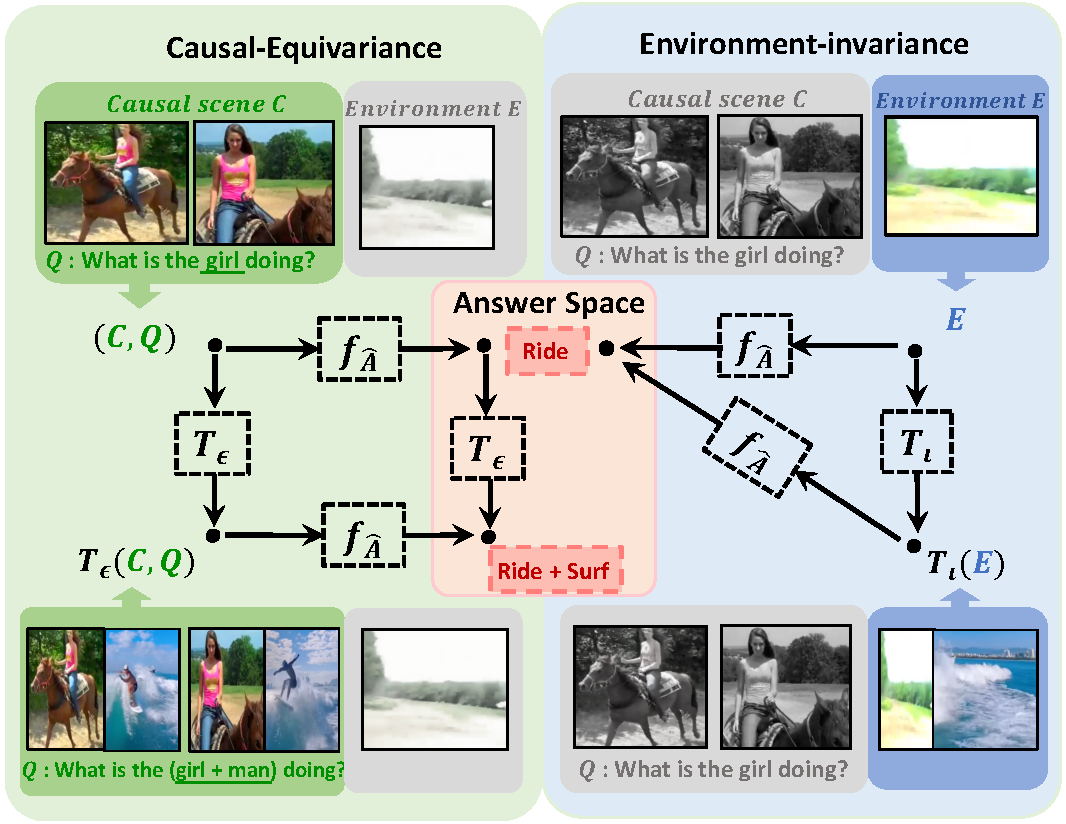
\includegraphics[scale=0.53]{fig/f1.pdf}
\caption{Illustration of causal-equivariant and environment-invariant principle, where $x$ is the input video-question pair, $f$ is a map from input space to answer space, $T$ is a transformation operator that applies to both input and answer space}.
% (\textcolor[rgb]{0,0.5,0}{Green}: causal-equivarince; \textcolor[rgb]{0.03,0.27,0.49}{Navy}: complement-invariance)}
\vspace{-5pt}
\label{fig:overview}
\end{figure}


% 2.problem of interpretable-------------------------------
% 第二段介绍explainability/interpretability in VideoQA:
% 一句话描述:对于black-box nature的concerns,explainability in VideoQA非常重要;
% 一句话描述:explainability in VideoQA是要回答什么问题:which part of the video should the model look at to answer the question?
% 然后说明现在都是post-hoc explanations,这里要点出来post-hoc的基本概念是啥;然后一两句话介绍post-hoc为啥有缺陷。

Trust concern on the black-box nature of existing methods calls upon a comprehensive study on model interpretability, \ie how they arrive at a specific prediction. 
%
In the context of the VideoQA, a favorable interpretation ought to answer the million-dollar question "which part of the video should the model look at to answer the question?" 
%
Despite the necessity, the explainability of the current design still dwells on the post-hoc paradigm \cite{gao2018motionappearance,DBLP:conf/iccv/Liu0WL21,10.1145/3474085.3475620}, where interpretations are approximated by extracting a salience pattern from the trained predictive model without any inductive knowledge ( \eg visualize attention weight).
%
Unfortunately, the visual justification via the post-hoc method is fragile against input perturbations, since some artifacts can be easily captured as explanations instead of genuine knowledge from the data \cite{DBLP:conf/ijcai/LaugelLMRD19}. As a result, peeking through output (\ie Grad-CAM \cite{DBLP:conf/iccv/SelvarajuCDVPB17}) is implicit and cannot faithful reveals how machine leverage the multi-modal information, which left our million-dollar concern unaddressed.

% which is fragile against input perturbations, and less instructive to the predictive mechanism. 


% In addition, it is debatable whether attention mechanisms are indeed explanations (Wiegreffe and Pinter, 2019; Jain and Wallace, 2019). M

% Worse still, overwhelming computational power has provoked the model complexity with billions of parameters, which, as a seed of distrust, shadowed the model's transparency along with our faith. 
%


% 3.partition the video to get interpretation ------------
% 第三段讲我们要研究的内容:
% 一句话介绍我们关注intrinsic interpretability,但是研究的人很少;
% 一句话描述我们的self-interpretable问题是“which part of the video is critical/causal to answering the question?”
% 然后引出我们要把visual scenes分成两部分一部分是causal scene,一部分是environmental scenes:分别介绍这两个具有啥子semantics。

Clearly, inferring a reliable rationale requires intrinsic interpretability to illuminate the reasoning insight. 
%
However essential, a self-interpretable VideoQA explainer that reveals such intrinsic prediction mechanism is until-now lacking.
%
To fill this gap, we get inspiration from \textit{causal theory} \cite{pearl2016causal} and capture such self-interpretability by answering the question of gold --- ``which part of the video is critical/causal to answering the question?'' 
% 
Concretely, we aim to find the causal part of input video on-the-fly that preserves the maximum visual information toward the question, whose discovery will justify the prediction and encourage the generalization.
%
Following this essence, one straightforward realization is to empower the model with discernment that grounds the visual scene into two segments: 
(1) \textbf{causal scene} that retains the question-critical video content and preserves all the relevant information about the target answer, which naturally serves as interpretation for the prediction; (2) \textbf{environment scene} that holds answer-irrelevant environment information of input video. 

% To the best of our knowledge, a self-interpretable VideoQA explainer that reveals the intrinsic prediction mechanism is critical to trustworthy videoQA but until-now lacking.
%

% Clearly, inferring a reliable answer requires a grounding rationale of the prediction, \ie to answer the million-dollar question "which part of the video scene should  be looking at?". 
%
% Inspired by the information bottleneck, which tends to reduce the overload of information processing \cite{DBLP:conf/iclr/SaxeBDAKTC18}, we aim to find the causal for input video that preserves the maximum visual information toward the question, whose discovery will justify the prediction and increase the generalization. 

%
% Following this essence, one straightforward solution is to empower the model with discernment that splits the visual scene into two segments: 
% (1) \textbf{causal scene} that retains the question-critical video content and preserving all the relevant information about the target answer, which naturally serves as interpretation for the prediction; (2) \textbf{environment scene} that holds answer-irrelevant environment information of input video. 


% 4.euiqvariant and invariant -------------------------------
% 要突出的是grounding,title中是Equivariant and invariant grounding,所以要让这些关键词尽早的出现。
% 这个例子融入到下面的Causal-Equivariance和Environmental-Invariance中去。
%
Discovering causal scene without fine-grained supervision is a luxury for VideoQA. Gazed upon the reasoning process, we argue the crux of this problem is to amplify the connection between the causal scene and the answer, while blocking the effect of the environment. 
%
Following this line, we put forward two principles to guide the grounding of the rationale.
%
% Following this line, we put forward \textit{Equivariance} and \textit{Invariance} principles to guide the grounding process.
% %
% Specifically, equivariance extends the model's sensitivity towards the a transformation $T$ on input $x$. Invariance, quite the contrary, inhibits the sensitivity and block model from input transformation. In light of this, the discovery of a stable rationale implies two requirements on the partition:
%
\begin{itemize}[leftmargin=*]
    \item \textbf{Causal-euqivariance.} 
    In essence, transformation on the causal scene should cause the parallel change on the representation manifold. By introspecting ``How would the predictive answer vary if the causal scenes change?'', the grounding mechanism is aware of the transformations and thus maintains the predictive interpretation.
    %
    As exemplified in Figure \ref{fig:overview}, equivariance implies that transformation applied to answer-critic information (\ie causal scene and question) should set off an equivariant semantic change in answer space.
    %
    Correspondingly, a cautious formulation of such co-variation should help the model pinpoint the 'girl-on-horse' scene as a grounding rationale for ``ride''.
    
    \item \textbf{Environment-invariance.} 
    % 是它不符合human cognition以及它会产生spurious correlation
    On the ground of the prophet, permutation on environment scene should be invariant to predictive answer, since environment implies no impact to the predictive answer except spurious correlation, comprising it as rationale runs counter to the human cognition. 
    % On ground of the prophet, the predictive answer is invariant against permutation on environment scene, as it does not contribute to the reasoning mechanism or interpretation.
    %
    Consider the example in Figure \ref{fig:overview} again, since an environment like ``landscape'' provides no evidence toward the answer ``ride'', its corresponding transformation should reflect a homogeneity in the answer space. The invariance principle epitomizes such assumption by ruling a transformation that is in-vary to answer permutation.
\end{itemize}


%5.overall idea ------------------------------------------------------------------
% Aspiring to capture grounding rationale, we formalize a model-agnostic learning framework, Equivariant and Invariant Grounding for Interpretable VideoQA (EIV), 
% %
% by asking the question ``what and how transformation should the model be equivariant or invariant to?'' 
% %
% Different from the previous effort that design supervised proxy task for geometric transformation \cite{DBLP:conf/iccv/ChengSM21}, 
% % we adopted philosophy of causal intervention and design a saliency-aware temporal mix method for the video input, and impose 
% we answer the ``what'' question by adopting the philosophy of causality \cite{pearl2009causal} and configure transformation as causal intervention operation that imposes scene-aware mixup \cite{DBLP:conf/iclr/ZhangCDL18} on the multi-modal input.
% %
% As for the question of how, we present a unified view of equivariant and invariant principles via the lens of temporal self-supervised learning, where the contrastive counterparts are bred through a disruption on the causal scene, environment scene as well as vision-language alignment.

% where the contrastive counterparts are bred through a disruption on the causal and environment scene, respectively.

% implemetation ----------------------------------------------
% 这一段的写作逻辑应该是如何实现equivariant、invariant principles的;可以不用follow IGV的写法;

% 可以这么组织:
% 一句话介绍三个modules;
% 然后如何用这三个modules来实现两个principle的:首先用grouidng indicator去roughly partition videos into two parts:causal and environmental scenes;然后基于这两部分引入causal-equivariance:利用interventer对于causal scenes做interventions,期望answer部分产生相对应的变化;利用interventer对于environmental scenes做interventions,期待这部分不会对于answering产生影响。
In light of the proposed princes, we formalize EIGV (\underline{E}quivariant and \underline{I}nvariant \underline{G}rounding for Interpretable \underline{V}ideoQA),
a model-agnostic explainer to capture the stable visual rationale VideoQA models.
% 一句话介绍三个modules;
Specifically, EGV absorbs three modules in addition to the backbone VideoQA model: a grounding indicator, an intervener, and a disruptor. 
%
%grounding indicator
In particular, the grounding indicator learns to separate the causal scenes as the interpretation and leave the rest as the environment. 
%
% causal-equivariance
Then, for the causal scene of interest, an intervener imposes the equivariance principle via a convex combination of two data points, while anticipating a corresponding change in the answer space.  
%
% environment-invariance
As for the environment counterpart, the invariant principle is realized using a similar intervener, but expecting an unchanged answer.
% %
% Noticeably, since mixing environment does not affect the reasoning dynamics, the answer is modified with the same ratio as the causal scene but independent to environmental one. 
%
% By capturing the equivariance from the answer to the causal scene and the invariance to environment, the model perceives a faithful interpretation that preserves the predictive mechanism.
%
On top of the intervened video, we present a unified view of equivariant and invariant principles via the lens of temporal self-supervised learning. 
%
Concretely, a disruptor substitutes the environment and causal scene with the stratification sampled from a memory bank (a collection of other training videos) to constitute the contrastive twins, respectively. 
%
% To fortify visual-question pair-wise cohesiveness, we also develops alternatives in addition to visual negatives by disrupting the visual-question coupling.
%
In addition to the visual negatives, we also develop alternatives by disrupting the visual-question coupling, to fortify their pair-wise cohesiveness.

% where the contrastive counterparts are bred through a disruption on the causal scene, environment scene as well as vision-language alignment.

% On top of the intervened video, the disruptor substitutes the complement scene with the stratification sampled from a memory bank (a collection of other training videos) and constitutes the “counterfactual video” as the positive sample.
% Likewise, the negative sample is constructed via replacement on the causal scene. 
% %
% In addition to the visual negatives that ``disrupt'' the causal scene, the disruptor also develops alternatives by disrupting the visual-question coupling, to fortify their pair-wise cohesiveness.
% 
After acquiring anchor representation alongside its contrastive twins, the auxiliary contrastive objective reveals the discriminative representation purely from the scene of interest, thus fostering the robustness of interpretation.

Briefly put, our contributions are: 
\begin{itemize}[leftmargin=*]
    \item We propose EGV, a model-agnostic VideoQA explainer that captures the intrinsic causal pattern in a self-interpretable manner.
    
    \item We investigate the soundness of grounding rationale by posing the equivariant-invariant principle on visual grounding and realize it via the causal instrument.
    
    \item We justify the superiority of EGV on three popular benchmark datasets (\ie MSVD-QA \cite{DBLP:conf/mm/XuZX0Z0Z17}, MSRVTT-QA \cite{DBLP:conf/mm/XuZX0Z0Z17},  NExT-QA \cite{DBLP:conf/cvpr/XiaoSYC21}) with extensive experiments, where our design outmatches all the state-of-the-art models.
\end{itemize}













